
Recent GDELT updates provide feeds with 15-minute resolution \cite{GDELT2}, but historical feeds offered only daily resolution. We decided for simplicity to analyze daily changes in price, taking a full day's worth of news data into account. This was most in line with testing our hypothesis, that an aggregation of topic clusters in a day's news is predictive of commodity pricing.

Our data pipeline was designed to provide day-wise parallelism over our data set in order to enable fast testing of new feature extraction methods. The raw data, as well as intermediate data, is stored in TSV ASCII format.

\subsection{Model}

Every news event in GDELT is stored as a row in a file for that day's report. Every set of rows may undergo a series of transformations. First, in the \textbf{preprocessing} stage, we extract relevant topic- and importance- related columns. For topics, a mix of numeric and categorical fields are extracted. Importance columns are saved for use in a further step. Next, in the \textbf{expansion} stage, we project each row of topic features to a purely real space by using one-hot encoding for categorical values. For each category, one-hot encoding produces $n$ dummy boolean variables, where $n$ is the number of unique categories. Finally, in the \textbf{summary} stage, $K$-means clustering is performed on this purely numeric representation of the data. Euclidean distance is used as the distance metric for $K$-means. Many clustering models are created with a range of $K$ from 10 to 5000. We use $K$-means for tractibility reasons.

The day summaries are then conglomerated in a time series $\{\textbf{d}_i\}$. For a day-indexed time series of a commodity's price, $\{p_i\}$, we have the corresponding sequence of binary labels indicating whether price has increased the next day, $y_i=1_{p_{i+1}>p_i}$.

Thus, our model assumes that:
\begin{enumerate}
\item The static clustering of news topics is accurate for the future.
\item $\mathbb{P}(p_{i+1}>p_i)$ may be determined by a regression over summaries $\textbf{d}_i$. 
\end{enumerate}

Both of these are strong assumptions. The first may be weakened by adapting a dynamic clustering model, such as an infinite Gaussian Mixture Model or a Hierarchical Dirichlet Process. The second requires $\textbf{d}_i$ to be both contain a sufficient amount of information to predict price behavior, which is a matter of appropriate feature extraction, and the assumption that we do not lose too much predictive power in summarizing a day by aggregating over the clusters to which its news events belonged.

\subsection{Execution}

Our current implementation uses $K$-means for clustering and logistic regression for classification. We trained, validated, and sampled from the days between 2006-01-01 and 2015-07-31. Recent days were used for testing.

For tractability reasons, we use a random sample of one million events to create the clustering models which are used in the main pipeline. This sample goes through the same preprocessing and expansion pipeline as the day summaries which are used in the regression except its output is used to create a clustering model. The sample is drawn uniformly from all events without any recency bias.

The raw data starts with $X=58$ columns. Each day has around $N=100,000$ rows, but this is variable between days. The total size of the set is about 60GB.

\begin{figure}[ht]
\vskip 0.2in
\begin{center}
\centerline{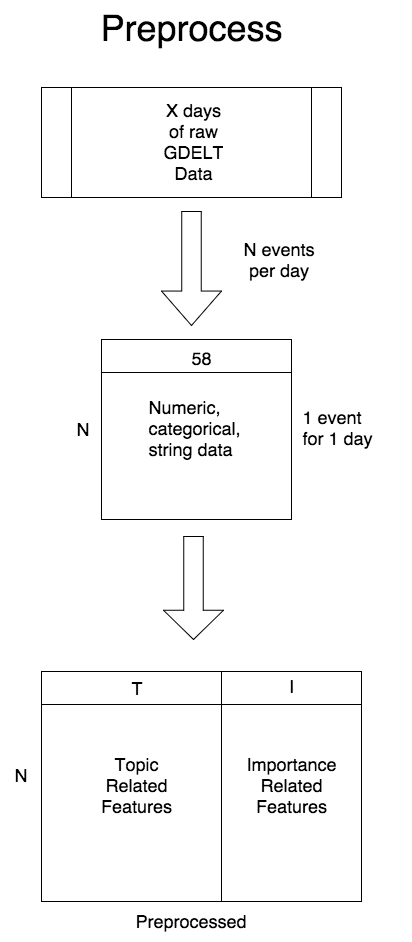
\includegraphics[scale=0.15]{images/preprocess_vertical.png}}
\caption{Preprocessing stage}
\end{center}
\vskip -0.2in
\label{fig:preprocess}
\end{figure}

The preprocessing step does standard data cleaning such as removing malformed rows but more importantly removes all but 19 of the original columns, and also groups the remaining into $T=12$ topic-related columns and $I=9$ importance columns. The removed columns have either redundant data or data deemed insufficiently relevant to commodity prediction. The topic columns are in a compressed format, with categorical variables represented as integers. String columns are sanitized and have stop words removed.

\begin{figure}[ht]
\vskip 0.2in
\begin{center}
\centerline{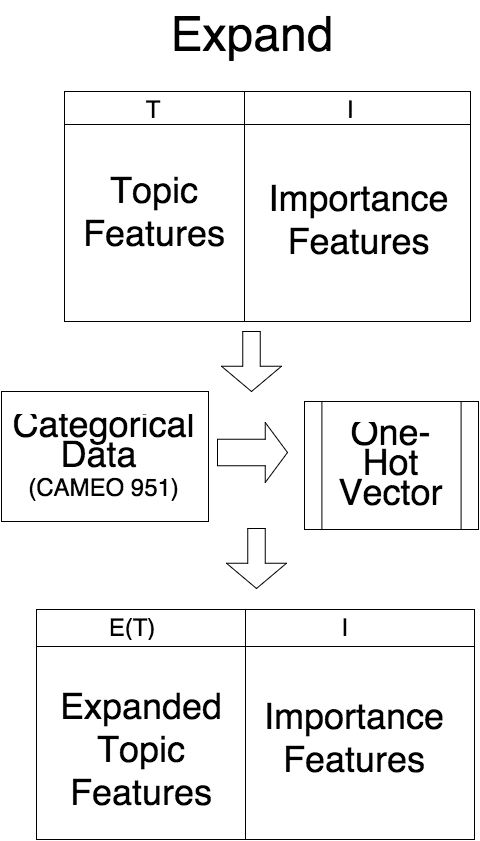
\includegraphics[scale=0.15]{images/expand_vertical.png}}
\caption{Expansion stage}
\end{center}
\vskip -0.2in
\label{fig:exapand}
\end{figure}

The expansion step one-hot encodes categorical features, such as the event CAMEO codes, producing $n$ dummy boolean variables, where $n$ is the number of unique categories. If the data for a categorical column is missing, its corresponding one-hot vector is the zero vector. The 19 feature columns are expanded to 938.


\begin{figure}[ht]
\vskip 0.2in
\begin{center}
\centerline{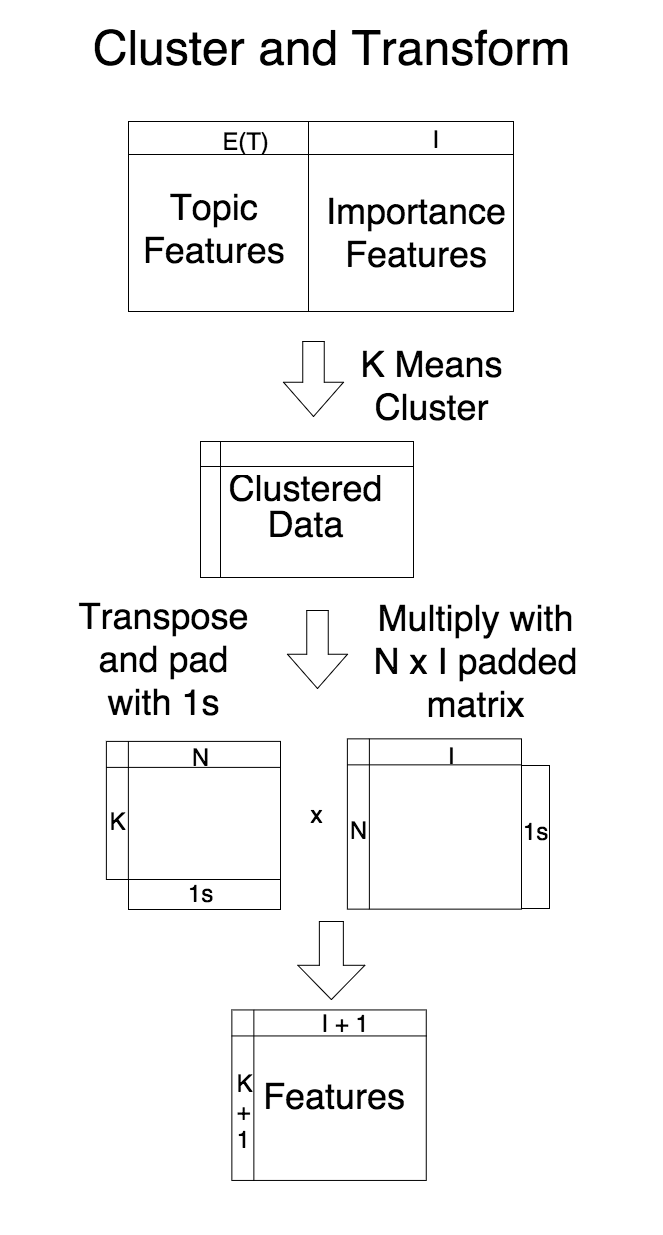
\includegraphics[scale=0.15]{images/cluster_and_transform_vertical.png}}
\caption{Summary stage}
\end{center}
\vskip -0.2in
\label{fig:summarization}
\end{figure}

As mentioned, the random sample is used to generate $K$-means models. These models are then used to cluster each day's data. We extract the $N$x$K$ clustered data and separate it into two matrices containing clustered topic data and clustered importance data and pad these matrices with $1$s, as in \ref{fig:summarization}. We then multiply the tranposed topic and importance matrices together. Because of the padded $1$s, their multiplication conveniently extracts the sum of importance-weighted events belonging to certain topics. Note that this model is extensible to a mixture model, where each event's contribution to a topic's importance for that day is weighed by the probability of belonging to that topic's class. Furthermore, the aggregation accomplished by the multiplication creates a highly reduced and uniform description of every day which is a flattened vector of dimension dependent on the cluster count.

These daily summaries are then enriched with historical pricing data before being fed into the linear model. The pricing data added are the 5, 10, and 30 day rolling averages of the commodity price. %TODO hyperparam selection of rolling mean.


\subsubsection{Autoregressive Models: ARMA}
We started our exploratory analysis with binary classification. We used diverse classification techniques such as Logistic Regression and Support Vector Machine on the sign of the change of the returns from a day to the next. The prices of silver from 2013 to 2015 were split between training, validation and testing in a 60:20:20 ratio. The best parameters from each model were chosen based on the validation accuracy. However, our test accuracy results were sub-par: Logistic Regression achieved a binary classification accuracy of 54.7\% and SVM achieved a binary classfication accuracy of 58.6\% . These models barely exceeded the baseline achieved by always guessing positive labels on the test set which would produce a 54\% accuracy. Therefore, we decided to employ Autoregressive models which combine the news data with the time series data in order to produce continuous predictions of next-day time series values.

Autoregressive models are some of the most flexible and easy to use models for time series. The future value of a variable, in an AR model, is assumed to be a linear function of several past observations and random errors. Accordingly, AR models have proven to be especially useful for describing the dynamic behavior of economic and financial time series and for forecasting \cite{tsay, VAR}. Recent literature proved their superiority in financial modeling, in terms of accuracy, to most other techniques such as Neural Nets and SVM. \cite{comparison} \\
The basic p-lag vector autoregressive model (AR(p)) has the form: $$\bf{Y}_t=\bf{c}+\bf{\Pi}_1\bf{Y}_{t-1}+\bf{\Pi}_2\bf{Y}_{t-2}+\cdots+\bf{\Pi}_p\bf{Y}_{t-p}+\epsilon_t,$$ $$t=1\ldots T$$ with $\Pi_i$ being the coefficients and $\epsilon_t$ is an unobservable zero mean noise. We can also do subset-autoregression where we pick multiple specific lags instead of a full range of lags like the basic AR(p) would do as show in the previous equation.\\
One of the most common extensions to Autoregressive models is to include moving averages and integration terms that take into account the stationarity of the time series. This is what constitutes Auto-Regressive Integrated Moving Average (ARIMA) models. They are  the most general class of models for forecasting a time series which can be made to be “stationary” by differencing (if necessary), perhaps in conjunction with nonlinear transformations.\\

Accordingly, an ARIMA model is fully determined by 3 parameters, one for each of the (AR),(I) and (MA) components:
\begin{enumerate}
	\item p = order of autocorrelation for (AR)
	\item d = order of integration (differencing) for (I)
	\item q = order of moving averages for (MA)
\end{enumerate}
Determining these orders can be done either visually using the Autocorrelation Function plot (finds the autocorrelation coefficients mentioned earlier) and the Partial Autocorrelation Function plot (correlation conditioned on other lags' autocorrelation) [Figure \ref{fig:ACF}] or analytically using a goodness of fit measure (which order fits the data best).\\
ACF or PACF plots indicates which lags are most correlated within the time series. They can be used to gauge if there is any sort of autocorrelation within the time series. They can be also be used to determine the exact orders depending on how the values in the plots decay or simply cut off but we're not covering those methods as we focused on the more methodical analytical approach.\\
\begin{figure}[ht]
	\vskip 0.2in
	\begin{center}
		\centerline{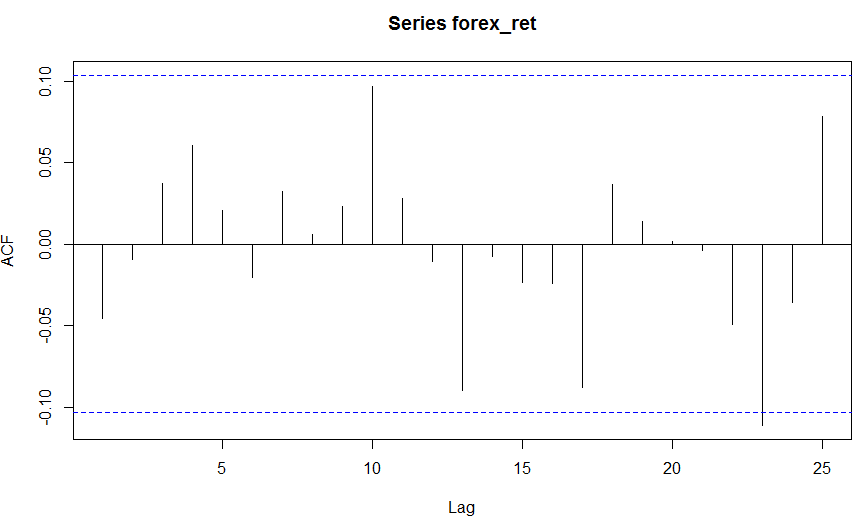
\includegraphics[width=\columnwidth]{ACF.PNG}}
		\caption{Autocorrelation Function plot for gold. Lags exceeding the dotted blue line have a statistically significant correlation with the 0-lag.Accordingly, the lags at 1, 14, 20 and 21 are correlated with the 0-lag (current time series).}
	\end{center}
	\vskip -0.2in
	\label{fig:ACF}
\end{figure}
For the goodness of fit, we had the options to use the Akaike information criterion (AIC), the Bayesian information criterion (BIC) or several other criteria that are more or less similar. These criteria would allow us to compare the goodness of fit of different models, indexed by their parameters. Accordingly, we would be able to decide the best order or parameters for our model based on the set that achieves the best fit. Later, we will discuss which subset of the data this fit was tested on.\\
For this paper, We decided to use the AIC: $$AIC = -2*\ln{L} + 2*k$$ where L is the maximum likelihood and k is the number of parameters. AIC aims to choose a model that minimizes the KL divergence between the true density and the density of the MLE of a fixed model.\\
Accordingly, the best model is the one with the lowest AIC. However, AIC is prone to overfitting and chooses predictive models over parsimonious ones. Given the literature's emphasis on the lack of predictive power in the domain of financial prediction, we decided to favor the predictive capacity over sparseness, for the order estimation, at least. BIC, on the other hand, favors sparsity over the predictive capabilities. \\
However, before testing the goodness of fit of different combinations of p and q parameters, we can figure out the d parameter using an Augmented Dickey Fuller test to verify the non-stationarity hypothesis of our data. Notice that random variable is stationary if its statistical properties are constant over time. Accordingly, it would have no trends and all of the variations around its mean would be random noise of constant amplitude. \cite{tsay, VAR}\\
If our data is already stationary, then there is no need for differencing (determining by the d component). In our case, for example, the non-stationary hypothesis was rejected with a p-value of 0.01 in the ADF test. Therefore, the d parameter that best fits our data is 0. \\
\subsubsection{Possible Extensions and Optimizations}
One possible extension to ARIMA or any time series model, for that matter, is adding a Markov Switching Model that assumes the existence of latent regimes and builds an independent model for each regime because.\cite{MS} After testing, we couldn't find any significant regimes in our training data which might infer that our regimes are over longer periods of time than that spanned by our data.\\
A possible optimization, which we benefited from, is the use of simple linear models (or generalized linear models) to simulate the AR component of ARIMA in case the (MA) component was deemed superfluous. In this case, we can build a simple design matrix where each column is a lagged version of the response variable. This design matrix can be used for a standard Ordinary Least Squares regressions as well as various other models that are computationally faster than ARIMA (with respect to their R implementations, at least).\\
\subsubsection{News Data: Exogenous Factors}
Our news data that we extract from GDELT is considered an exogenous factor. In the time series literature, there have been several approaches to including such information into time series models. The most two prominent methods are impulse responses or simply considering the exogenous data as time series to be evaluated alongside the financial times series (the way you'd do in a regression) such as in ARIMAX models (ARIMA + Exogenous).\\
The impulse response method attempts to detect impulses, whose response or effect decays with time,  within the time series data in order to localize the date of origin. Consequently, one would try to match the dates of such impulses with our news data in order to detect which columns in our data are most correlated with the big changes in those dates.\\
ARIMAX is simpler and more efficient, in literature and from our experience, especially with our linear models simplification. We add the columns of the news as extra time series whose autocorrelation with the response variable is evaluated in training. Note however that we use a lagged version of the news since our hypothesis is that the news from day D would affect the market after day D's closing which will be reflected on the difference of the values between D+1 and D.\\
\subsubsection{Column Selection of News Data}
However, a large number of columns in the news data (800 in the case of 100 clusters of GDELT data) can easily cause overfitting since the large number of variables could fit arbitrary data points to the noisy news columns. Accordingly, our out-of-sample testing results would suffer.\\
Another problem with a large number of columns is that ARIMA (the original implementation) and Ordinary Least Squares regression require the number of features to be less than or equal to the number of observations. This can be limiting as we would like to test different numbers of training days. Therefore, we recurred to Principal Component Analysis (among other methods that we tried) to reduce the dimensions. PCA converts a set of observations of possibly correlated variables into a set of values of linearly uncorrelated variables called principal components.\cite{PCA} One can select a fixed number of principal components that express most of the variance in a certain data set. In our case, we selected a number of principal components that accounted for $99\%$ of the variance in our data and used those principal components of the news data for the training as exogenous factors, instead of the original news columns. \\
\subsubsection{L1-regularization: Lasso Regression}
We also tried L1-regularization with Lasso regression since it inherently handles overfitting by enforcing sparsity, as compared to preemptively regularizing based on the variance, as in the case of PCA. \cite{glmnet}
\begin{figure}[ht]
	\vskip 0.2in
	\begin{center}
		\centerline{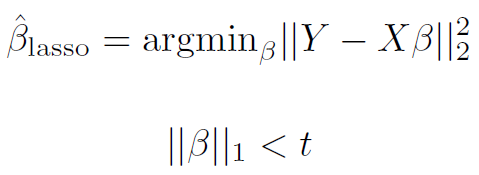
\includegraphics[scale=0.15]{Lasso.PNG}}
		\caption{Lasso Regression}
	\end{center}
	\vskip -0.2in
	\label{fig: Lasso}
\end{figure}
Lasso is a least-squares regression with an L-1 penalty to minimize the L-1 distance of the regression coefficients. Accordingly, Lasso is sparse since many elements of the array of coefficients is 0. Therefore, it eliminates the least important regressors. Accordingly, Lasso's sparsity is based on the actual importance of each regressor or news column with respect the response variable. The implementation (GLMNET), consequently, doesn't require the number of variables to be less than the observations which allows us to test a small number of observations without applying any dimension reduction beforehand. \cite{glmnet}\\
Additionally, Lasso is computationally efficient as compared to other sparse regressions.\cite{glmnet} Finally, we can select the degree of our sparsity by selecting a Lambda coefficient which helps us better gauge the change of the predictive power of our model. \\
Accordingly, we build Lasso model with the minimum Lambda as defined by cross-validation and then use that model to estimate our log-returns for each training window. \\
\subsubsection{Testing Measures}
For out-of-sample testing, we used two measures to evaluate the predictive capacity of the model and if it suffers from bias caused by the training data. The first is Mean Absolute Error which describes the difference in absolute value between our predictions and actual values. The closer MAE is to 0, the better we fit the data quantitatively. However, for our final purpose of designing a trading strategy, it could be good enough to detect if the stock is going up or down. In this case, predicting the binary values is what we seek. Accordingly, we would convert our predictions to binary based on their sign (positive log returns implies an increase from last day) and use simple binary-classification measures such as the accuracy rate. We focused on the accuracy rate because we have almost equal amount of positive and negative data points that we are not biased by the training which is usually the reason for evaluating recall, precision and F-1 measures.\\
\subsubsection{Training the Time Series}
The time series we had most success with is the spot price of Silver, in US Dollars between the dates of January 1st, 2013 and June 1st, 2015. We also converted our price values into log-returns as a way to normalize the values such as we model and forecast the log of the change rather than the values themselves. This is a common practice in financial modeling since it makes computations more efficient and comparison to other literature easier (scale independent). \cite{tsay} 
$$LogReturn = \log{\frac{X_t - X_{t-1}}{X_{t-1}}}$$
We split our data into training and testing windows of varying sizes as can be seen in the results section. The windows guarantee the temporal order of the data points which is important for a time series analysis. We also resorted to a moving window technique, also called walk-forward optimization, which is a form of k-fold cross-validation for time series data. In this technique, we would slide the window on the training set of the time series data and re-estimate the coefficients at each iteration then look ahead by 1-step instead of multiple steps. Note that we're not re-estimating the order as we opted for estimating the order only once for the whole training dataset. This decision was motivated by the assumption that the order would be more or less constant over our small-to-medium range of dates and that re-computing it would be expensive and problematic to any future online implementations of this model or system.\\
Note that moving-window training is expected to have a higher predictive power than a simple fixed window technique since the model changes as the window moves and thus holds more significance as the predictions go further in time. With a fixed window, the further the predictions are from the window, the less relevant is the model from the fixed window since it's based on data that is too old. \\
Finally, we then collect the mean absolute error and the binary accuracy over all the iterations (different windows) and average them to evaluate the model for a given hyper-parameter. In our case, the main hyper-parameters was the size of the training window.\\

